%%%%%%%%%%%%%%%%%%%%%%%%
%
% $Author: Achal Shakywar, Malik Al Ashter Ghansletwala$
% $Date: 2024-01-24  $
% $Shodrt The content list details the software components used in the project, including the Arduino IDE, Arduino Library for Nano 33 BLE Sense, TinyML model development tools, audio processing libraries, machine learning frameworks, Python, and tools for documentation and version control. It also discusses any software or environment constraints. $
% $Directory: ML23-01-Keyword-Spotting-with-an-Arduino-Nano-33-BLE-Sense/report/Contents/en/SoftwareDescription.tex $
% $Version: 5.0 $
% $Review by: $
% $Review date: $
%
%%%%%%%%%%%%%%%%%%%%%%%%

\chapter{Software Description}

To implement a TinyML project for keyword spotting using an Arduino Nano 33 BLE Sense, several software components and tools are necessary. Here's an overview:

\section{Arduino IDE Description}\label{ArduinoIDE}

It is an open source official Arduino software which used for editing, uploading and
compiling codes in to the Arduino module. It is a cross-platform software which is
available for Operating Systems like Windows, Linux, macOS. It runs on Java platform
and supports a range of Arduino modules. It supports C and C++ languages. The
microcontrollers present on the Arduino boards are programmed which accepts the
information in the form of code. The program written in the IDE is called a sketch
which will generate a Hex file which is then transferred and uploaded in the controller.
The IDE environment is made up of two parts: an editor and a compiler. The editor
is used to write the required code, while the compiler is used to compile and upload
the code to the Arduino Module.\cite{Fezari:2018}
The Menu bar has options such as File in which there are many options including
Opening a new file or existing, Examples-in which we can find sketches for different
applications like Blink, Fade etc. There is an error console at the bottom of the screen
for displaying errors.

The 6 buttons are present on top of the screen are as follows:

\begin{figure}[H]\centering
	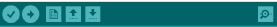
\includegraphics[width=8cm]{Images/software/MenuButton}
	\caption{\textbf{Menu Button.}}
	\label{fig:MenuButton}		
\end{figure}


\begin{itemize}
	\item	The check mark is used to verify your code. Click this once you have written your code.
	\item	The arrow uploads your code to the Arduino to run.
	\item	The dotted paper will create a new file.
	\item	The upward arrow is used to open an existing Arduino project.
	\item	The downward arrow is used to save the current file.
	\item	The far right button is a serial monitor, which is useful for sending data from the Arduino to the PC for debugging purposes.
\end{itemize}

\subsection{Installation}
\label{Arduinoide}
To install the Arduino IDE, we need to download the latest version from the Arduino webpage \url{https://www.arduino.cc/en/software}. We can select the version based on the operating system we are using. Here we are installing Arduino 1.8..15 for a Windows 10 operating system. 
The set up file name is arduino-1.8.15-windows.exe and the size of it is 1,17,470 KB. we can specify the path according to our needs. Here the path is set as  \SHELL{C:/Program Files (x86)/Arduino}.

\begin{figure}[H]\centering
	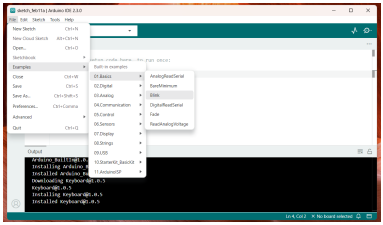
\includegraphics[width=8cm]{Images/software/MenuBarOption}
	\caption{\textbf{Menu Bar Option}}
	\label{fig:MenuBarOption}		
\end{figure}

After the download is done, open the setup file and proceed to install.
Select all the components in the dialog box and click Next.

Select the destination folder and click Install





Once the installation is done, open the Arduino IDE and a default sketch appears on the screen as shows.

\begin{figure}[H]\centering
	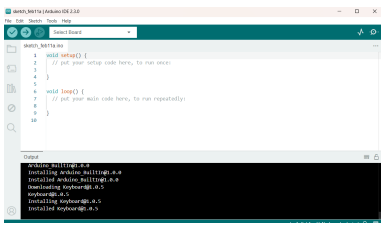
\includegraphics[width=8cm]{Images/software/ArduinoIDESketch}
	\caption{\textbf{ArduinoIDESketch}}
\label{fig:ArduinoIDESketch}		
\end{figure}


It can be seen from the above figure that the basic arduino sketch has two parts. The first part is the function \PYTHON{void setup()} which returns void and we do the intiliaztion such as the output LED color, specifying the core etc. The second part is the function \PYTHON{void loop()} where we define functions which are to be performed through out the loop. These codes are placed between paranthesis \PYTHON{$\{ \}$} and each function has a return type, here it has void return type.

\subsection{Arduino IDE on PC}
\subsubsection{Installation}
Arduino Nano 33 BLE Sense uses the Arduino software integrated development environment (IDE) for programming, which is the most widely used and common (IDE) for all arduino boards that can be run online and offline. This is a open-source Arduino Software (IDE) makes it easy to write code and upload it to the board. There are various version of software which is supported for each operating system (OS) e.g: mac, linux, and windows. Arduino community also provide us to start coding online and save our sketches in the cloud, this online arduino editor is most up-to-date version of the IDE includes all libraries and also supports new Arduino boards. For getting access to these software packages go to the following link \url{https://www.arduino.cc/en/software}  and get more up to date inforamtion, because every single day there are some updates occurs which is available on the link mention above. These software can be used with any Arduino board, the most recent offline arduino IDE 1.8.15 can be seen in Figure,\ref{fig:ArduinoCreat AgentInstallation}. it is also supportive for all operating systems.


\begin{figure}[H]\centering
	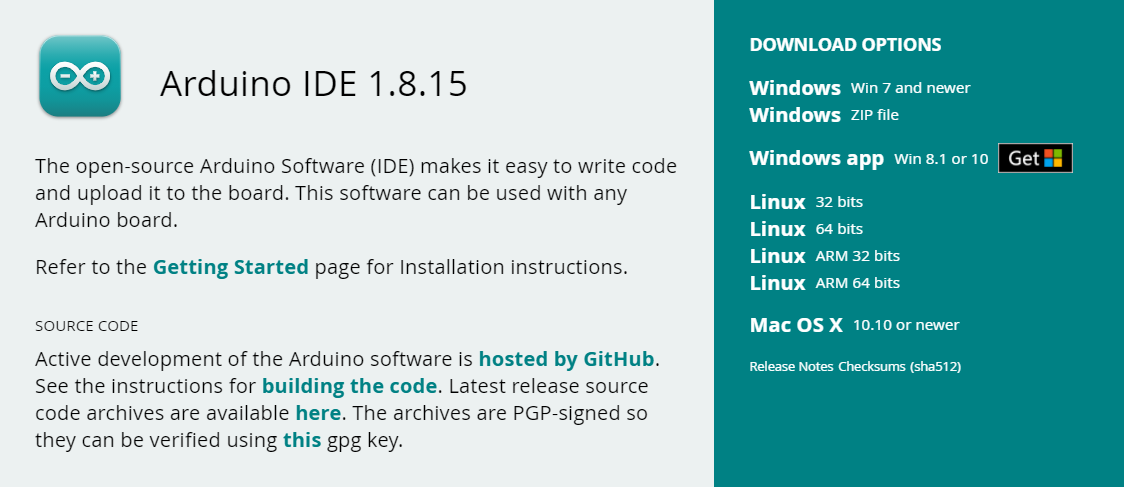
\includegraphics[width=8cm]{Images/software/ArduinoCreatAgentInstallation}
	\caption{\textbf{Arduino Creat Agent Installation}}
	\label{fig:ArduinoCreatAgentInstallation}		
\end{figure}

\subsection{Configuration}
\subsubsection{Configuration for the Arduino Nano 33 BLE Sense}
To program the Arduino Nano 33 BLE Sense in offline state, we need to install one
of the latest arduino IDE on our desktop. After installation, for getting access to
the Arduino nano 33 ble sense board, we need to make configuration in our IDE. By
opening the IDE, go to tool which can be seen on the uper left corner in IDE, in the
tool there is an option for managed board. At this point we need to write our board
name in the search which is Arduino Nano 33 BLE Sense as shown in figure,\ref{fig:ArduinoMbedOSNanoBoardsInstallation}.Select
the Arduino Mbed OS Boards and install it. The Mbed OS nano board supports also
other nano family boards including Arduino nano 33 ble sense, after installing simply
connect the Arduino Nano 33 BLE Sense to the computer via USB cable.


\begin{figure}[H]\centering
	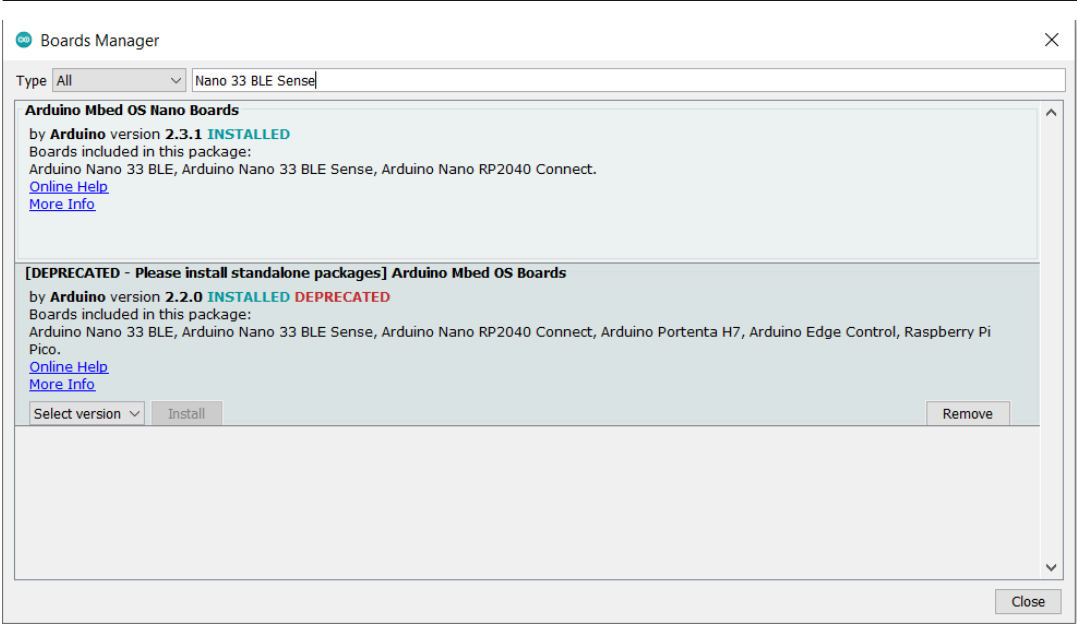
\includegraphics[width=8cm]{Images/software/ArduinoMbedOSNanoBoardsInstallation}
	\caption{\textbf{Arduino Mbed OS Nano Boards Installation}}
	\label{fig:ArduinoMbedOSNanoBoardsInstallation}		
\end{figure}


\subsection{Setup}
There are set of examples which are build in Arduino (IDE) for the testing purpose, for checking all the configuration and setting up the board we can open one of the basic LED blink example first as shown in the figure.  


\begin{figure}[H]\centering
	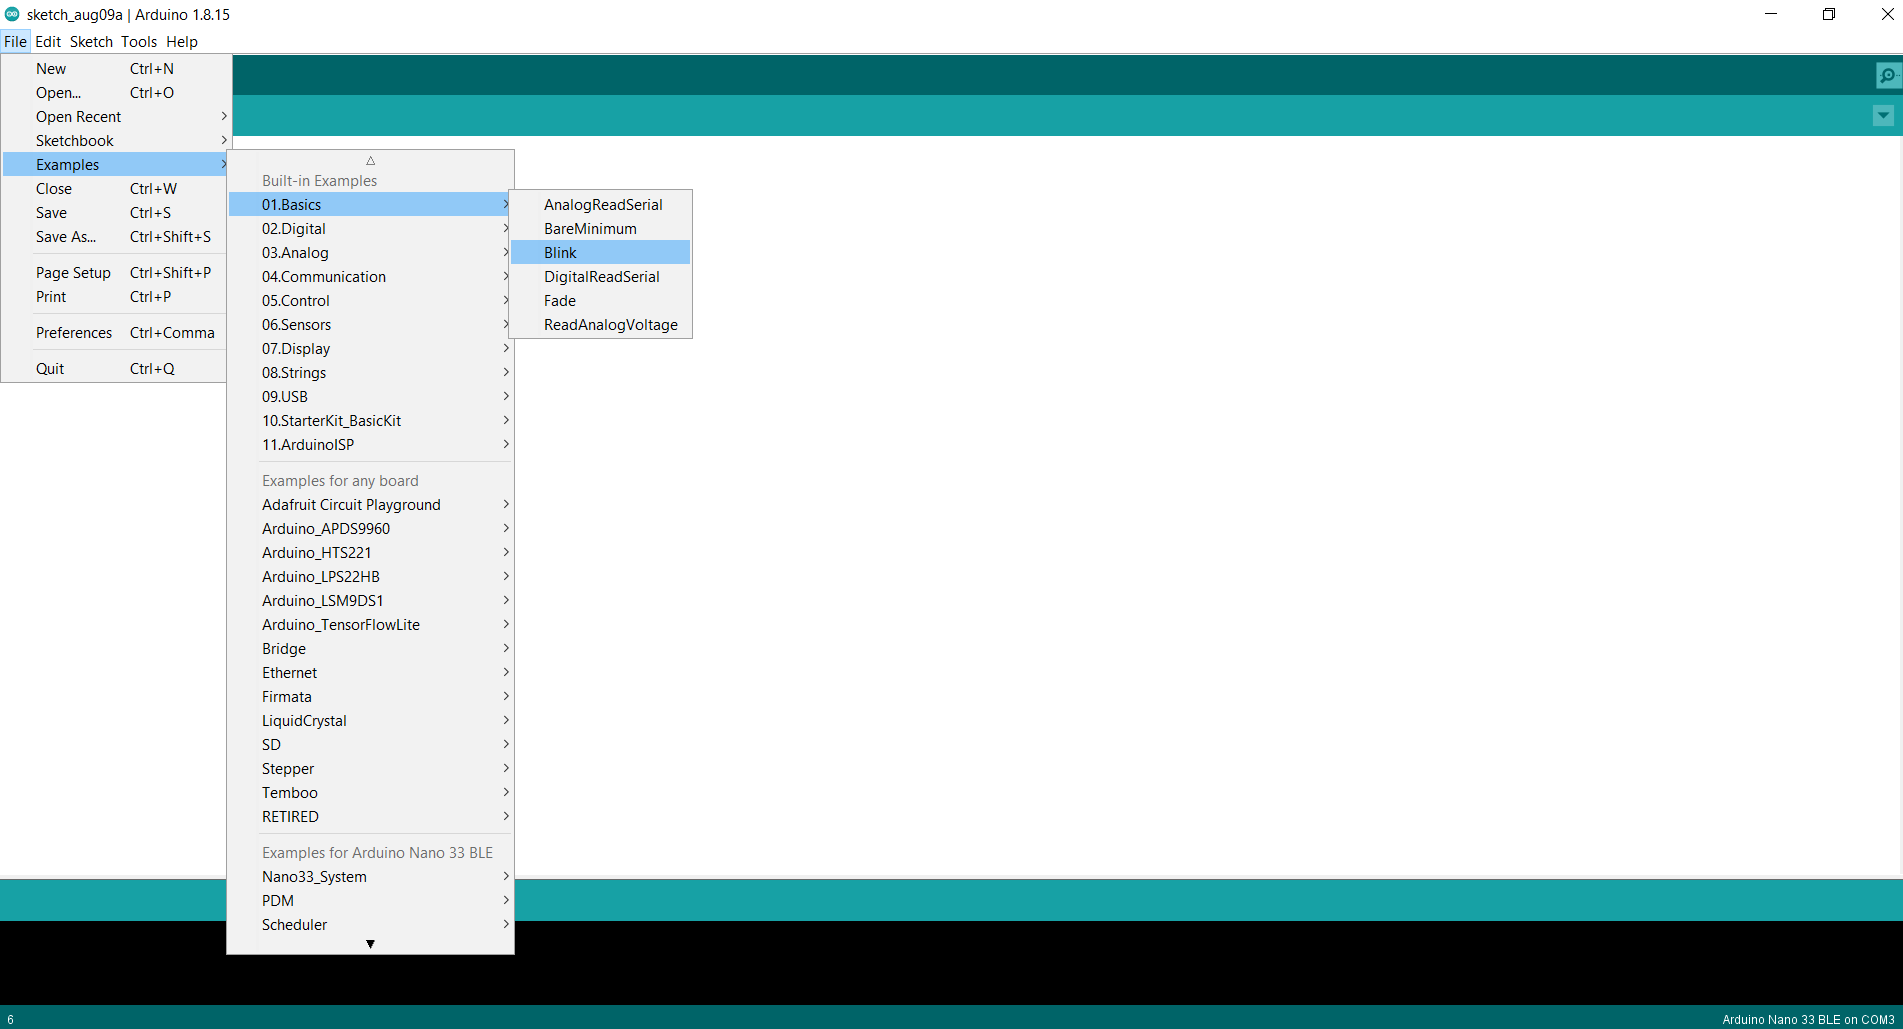
\includegraphics[width=8cm]{Images/software/SetupTest}
	\caption{\textbf{Setup Test}}
	\label{fig:SetupTest}		
\end{figure}


This LED-blink example support all the arduino boards, for the checking purposes just need to run this basic example on any arduino embed board and it will blink the LED on our Arduino board after pre-set miliseconds. In the same example folder, there are also number of build in usefull example written in Arduino IDE for embedded boards. These examples are very usefull for getting the basic knowledge about the board and programming.

\subsection{constraints}
There are some pre-requisite steps need to follow either we need to run the build in example or run by our own written program. By operating the Arduino board with Laptop with the help of USB connection, need to open the Arduino IDE on desktop, it appears a blank arduino environment page just a Void setup and void loop written on it. At this step we need to go to the tool-Arduino board and select the connected board which is Arduino Nano 33 Ble Sense as shown in the figure.

\begin{figure}[H]\centering
	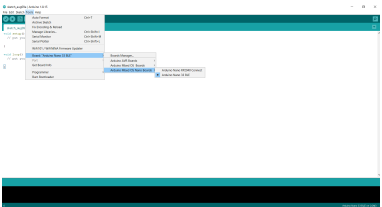
\includegraphics[width=8cm]{Images/software/SelecttheConnectedboardhereArduinoNano33}
	\caption{\textbf{Select the Connected board here Arduino Nano 33}}
	\label{fig:SelecttheConnectedboardhereArduinoNano33}		
\end{figure}

\subsubsection{Select the Appropriate Port}
By selecting the Arduino nano 33 BLE sense board, next we need to check the connected port. For doing this, we need to set our arduino borad in Boot setup by clicking the white reset button on arduino as show in figure.

\begin{figure}[H]\centering
	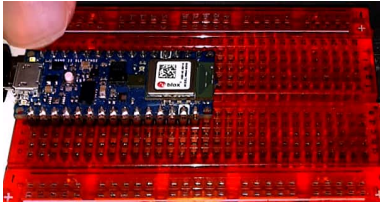
\includegraphics[width=8cm]{Images/software/ArduinoNano33BLESenseResetButton}
	\caption{\textbf{Arduino Nano 33 BLE Sense Reset Button}}
	\label{fig:ArduinoNano33BLESenseResetButton}		
\end{figure}


After successfully applying the above mention step, next we need to select the connected
port before upload the program. For this, go to tool select arduino port and make
sure to check it available port for uploading the program as shown in figure\ref{fig:Select Available Port for Uploading Arduino Sketch}

\begin{figure}[H]\centering
	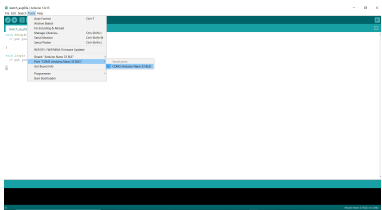
\includegraphics[width=8cm]{Images/software/SelectAvailablePortforUploadingArduinoSketch}
	\caption{\textbf{Select Available Port for Up loading Arduino Sketch}}
	\label{fig:SelectAvailablePortforUploadingArduinoSketch}		
\end{figure}

\subsection{Data quality}

The Arduino Integrated Development Environment (IDE) is a key component in the Magic Wand project with Arduino Nano 33 BLE Sense. Here’s a detailed explanation of its quality aspects.\cite{Fezari:2018}

\begin{enumerate}
	\item \textbf{Ease of Use}: The Arduino IDE is user-friendly and designed to be easy to use for beginners, while also providing advanced features for experienced users.
	
	\item \textbf{Cross-Platform Compatibility}: The Arduino IDE is compatible with Windows, macOS, and Linux, making it accessible to a wide range of users.
	
	\item \textbf{Open-Source}: The Arduino IDE is open-source, which means its source code is freely available. This allows for community contributions, leading to continuous improvements and updates.
	
	\item \textbf{Support for Multiple Boards}: The Arduino IDE supports not only the Arduino Nano 33 BLE Sense but also a wide range of other Arduino boards.
	
	\item \textbf{Built-In Code Editor}: The Arduino IDE comes with a built-in code editor that provides features like syntax highlighting and automatic indentation, making it easier to write and debug code.
	
	\item \textbf{Library Manager}: The Arduino IDE includes a Library Manager that makes it easy to install and manage libraries. This is particularly useful for the Magic Wand project, which requires libraries like TensorFlow Lite for Microcontrollers.
	
	\item \textbf{Serial Monitor}: The Arduino IDE includes a Serial Monitor that allows you to monitor data sent from the Arduino Nano 33 BLE Sense in real-time. This is crucial for the Magic Wand project, as it allows you to monitor the gesture recognition process.
	
	\item \textbf{Community Support}: The Arduino IDE has a large and active community. This means you can find a wealth of tutorials, guides, and troubleshooting advice online.
\end{enumerate}


\subsection{Data quantity}
Magic Wand project with Arduino Nano 33 BLE Sense, “Data Quantity” in the software description of the Arduino IDE refers to the amount of data that the software can handle or process. Here’s a detailed explanation:
\begin{enumerate}
	\item \textbf{Code Size}: The Arduino IDE needs to handle the code for the keyword spotting project. This includes the code for collecting and processing sensor data, running the machine learning model, and any additional functionality.
	
	\item \textbf{Library Size}: The Arduino IDE also needs to handle various libraries that are used in the project. This includes the TensorFlow Lite for Microcontrollers library, which is used to run the machine learning model on the Arduino Nano 33 BLE Sense.
	
	\item \textbf{Sensor Data}: The Arduino IDE needs to handle the sensor data that is collected by the Arduino Nano 33 BLE Sense. In one experiment, a window size of 2 seconds was used, which means 200 rows of accelerometer data or 600 values of x, y, and z acceleration axis were fed into the model.\cite{Fezari:2018}
	
	\item \textbf{Model Data}: The Arduino IDE needs to handle the data of the machine learning model. This includes the model parameters and the model output.
	
	\item \textbf{Data Transmission}: The Arduino IDE also handles data transmission between the Arduino Nano 33 BLE Sense and the computer. This includes uploading the program to the board and transmitting sensor data and model output to the computer for monitoring.
\end{enumerate}

\subsection{Data types}

\begin{itemize}
	
	\item \textbf{Software Components:}
	\begin{itemize}
		\item \textbf{TensorFlow Lite For Microcontrollers:} This is an optimized version of TensorFlow, targeted to run TensorFlow models on tiny, low-powered hardware such as microcontrollers. It doesn't require operating system support, any standard C or C++ libraries, or dynamic memory allocation.
		\item \textbf{Arduino IDE:} This is the software used to write and upload computer code to the physical board.
	\end{itemize}
	
	\item \textbf{Data Types:} You'll likely be working with arrays to store the sensor data, and you'll use TensorFlow Lite's data types for the model's input and output. The exact data types will depend on your specific implementation and the requirements of the TensorFlow Lite model.
\end{itemize}


\begin{enumerate}
	\item \textbf{Numeric Data Types:}
	\begin{itemize}
		\item Identify the numeric data types used, such as integers, floating-point numbers, or doubles.
		\item Describe the range and precision of each numeric data type.
	\end{itemize}
	
	\item \textbf{Text Data Types:}
	\begin{itemize}
		\item Specify if the software handles text data, such as strings or characters.
		\item Discuss any character encoding or formatting requirements.
	\end{itemize}
	
	\item \textbf{Sensor Data Types:}
	\begin{itemize}
		\item If interacting with sensors, specify the types of sensor data used.
		\item Describe the format and units of measurement for each sensor data type.
	\end{itemize}
	
	\item \textbf{Custom Data Types:}
	\begin{itemize}
		\item Discuss any custom data types defined in the software, such as structs or classes.
		\item Explain the purpose and structure of each custom data type.
	\end{itemize}
	
	\item \textbf{Data Conversion and Casting:}
	\begin{itemize}
		\item If data conversion or casting operations are performed, describe how different data types are converted or casted.
	\end{itemize}
	
	\item \textbf{Data Representation:}
	\begin{itemize}
		\item Explain how data is represented, including binary, hexadecimal, or other representations.
	\end{itemize}
\end{enumerate}



\subsection{Data structure}

\begin{itemize}
	
		\item \textbf{Data Structures:}
	\begin{itemize}
		\item \textbf{Sensor Data:} The Arduino Nano 33 BLE Sense collects sensor data, which is multidimensional and complex. This data is typically stored in arrays or similar data structures for processing.
		\item \textbf{Model Input and Output:} The sensor data is passed to the TensorFlow Lite model as input, and the model outputs a simple classification. The exact data structures for these will depend on the requirements of your TensorFlow Lite model.\cite{Harris:2023}
		
	\end{itemize}
\end{itemize}




\begin{enumerate}
	\item \textbf{Arrays:} Used to store a collection of data items of the same type. Example: storing sensor readings over time, storing LED brightness levels.
	
	\item \textbf{Structures (\texttt{struct}):} Allows grouping multiple variables of different types under a single name. Example: defining a struct to hold sensor data (e.g., temperature, humidity).
	
	\item \textbf{Classes:} Used for creating user-defined data types with properties and methods. 
	
	\item \textbf{Linked Lists:} Data structures consisting of a sequence of elements where each element points to the next element. Example: implementing a linked list to manage a queue of actions to perform.
	
	\item \textbf{Stacks:} Last in, first out (LIFO) data structures where elements are inserted and removed from the same end. Example: using a stack to manage function calls or nested operations.
	
	\item \textbf{Queues:} First in, first out (FIFO) data structures where elements are inserted at the end and removed from the front. Example: implementing a queue for handling incoming commands or tasks.
	
	\item \textbf{Trees:} Hierarchical data structures consisting of nodes connected by edges. Example: representing hierarchical data such as menu structures or organizational charts.
\end{enumerate}



\subsection{Conclusions}
\subsubsection{Output Window (Serial Monitor)}
Serial Monitor is the another window on the Arduino IDE, which shows the Input/Output of our program and results appear on it as per the required output. For getting
access to Serial monitor, we need to go extreme right in the Arduino IDE, the small
circle pop up when we reach it is the serial monitor as show in the figure.

\begin{figure}[H]\centering
	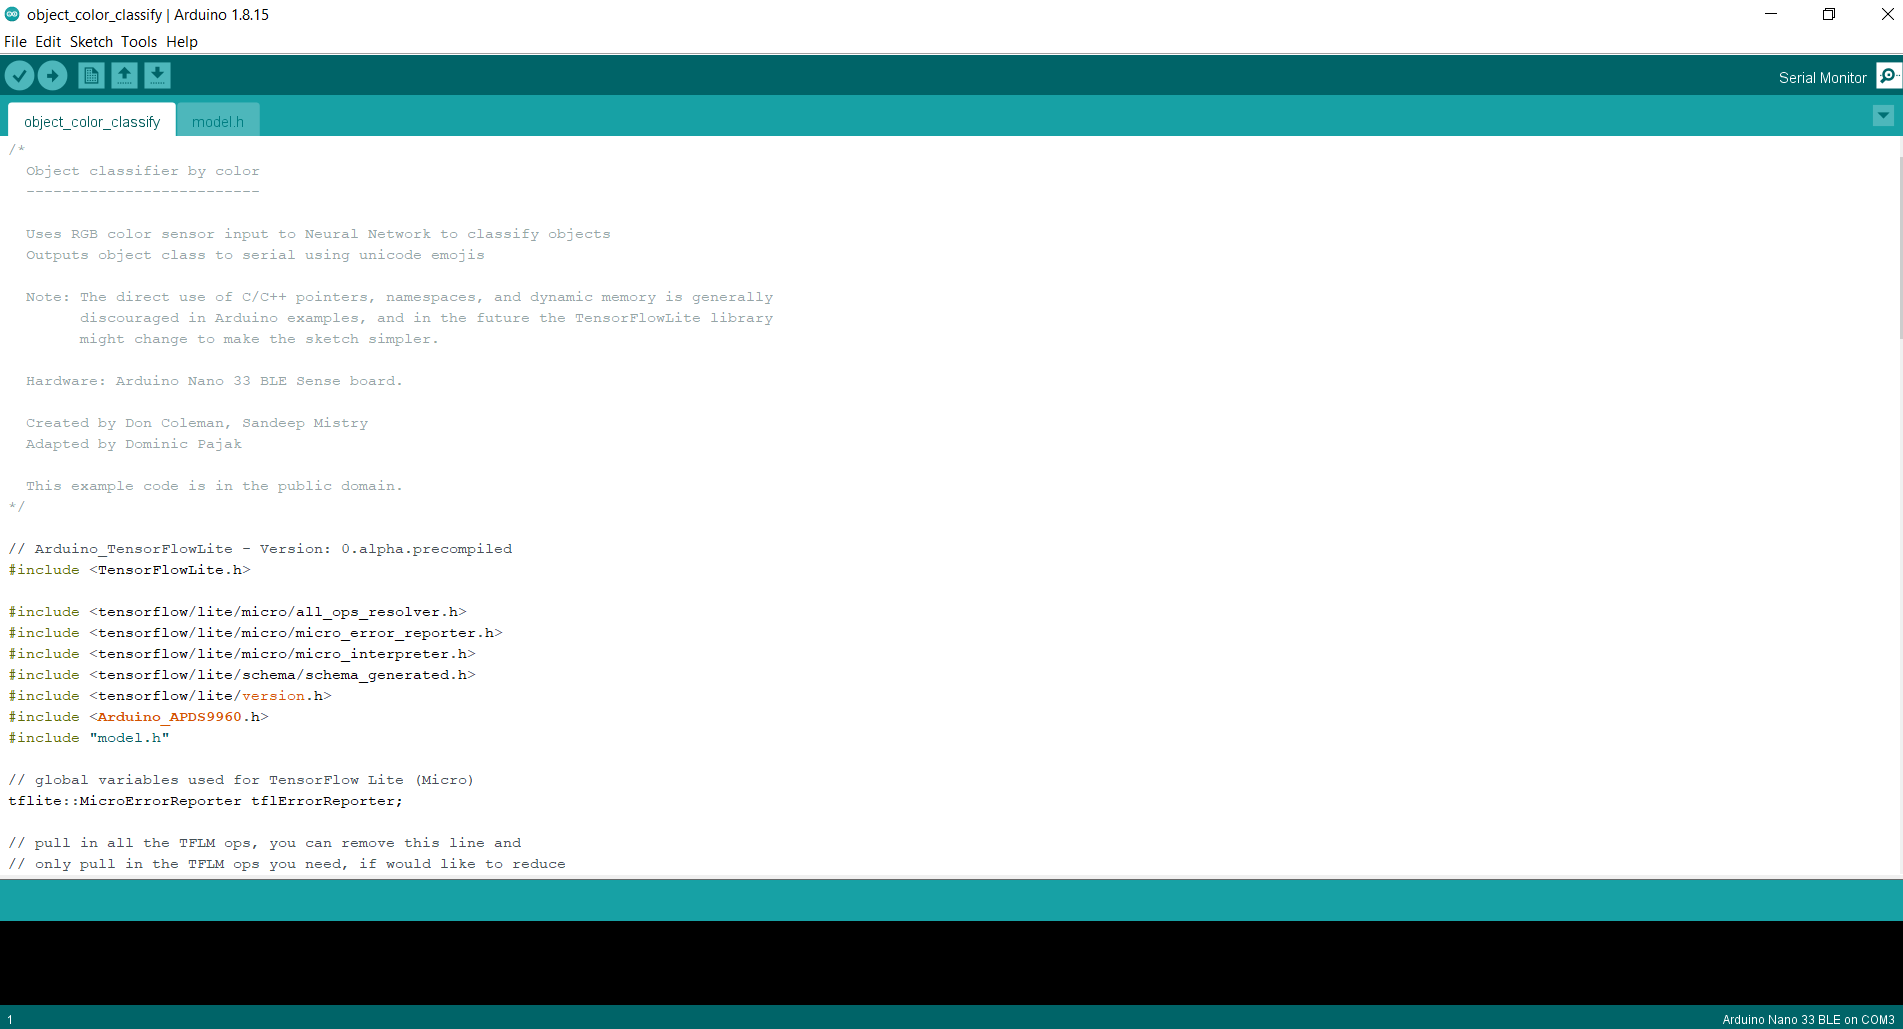
\includegraphics[width=8cm]{Images/software/SerialMonitor}
	\caption{\textbf{Serial Monitor}}
	\label{fig:SerialMonitor}		
\end{figure}
 
The Final results, all the variables, input, sensor values are shown in the serial monitor
the (Output Window) as shown in the figure by clicking the serial monitor button.

\begin{figure}[H]\centering
	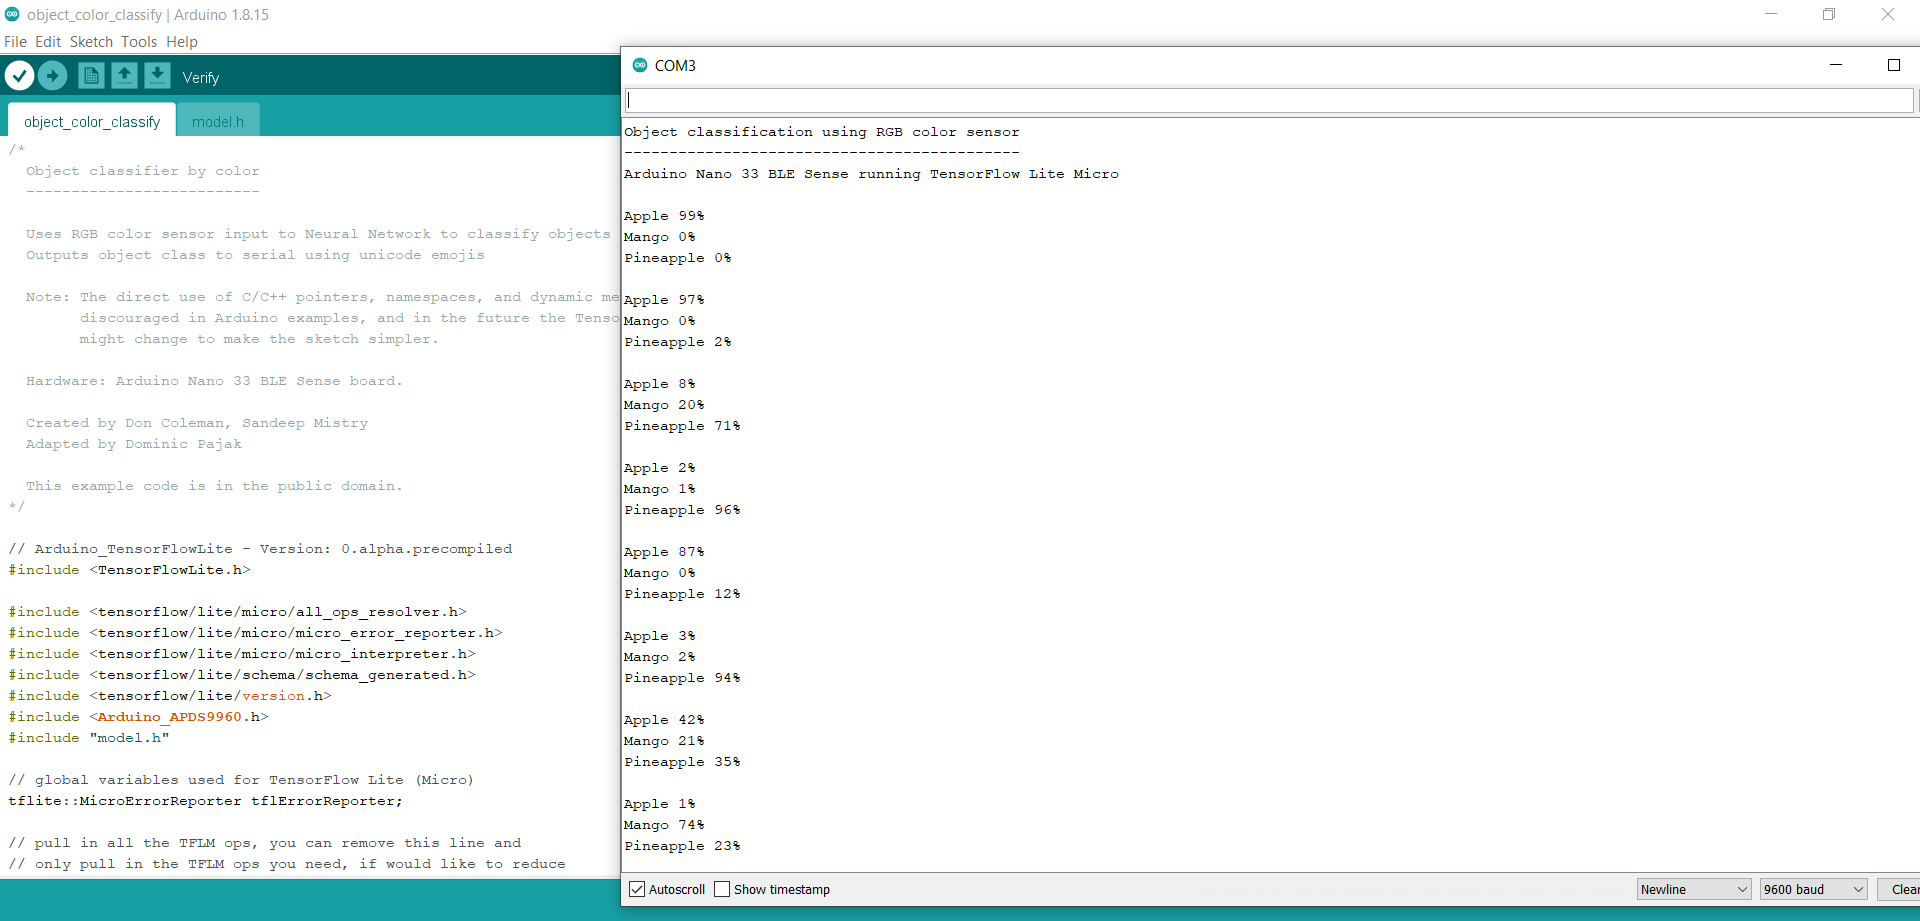
\includegraphics[width=8cm]{Images/software/OutputWindow}
	\caption{\textbf{Output Window}}
	\label{fig:OutputWindow}		
\end{figure}

\section{TensorFlow}
\label{TensorFlow}

TensorFlow is an end-to-end, open-source platform popularly used for the quick implementation of machine learning algorithms. A rich ecosystem of tools, libraries, and community resources has made it extremely popular among machine learning researchers and practitioners to develop and deploy various machine learning algorithms with greater efficiency and flexibility. TensorFlow has become popular in recent times for the quick development of complex deep neural network architectures for both experimentation and developing production-ready software.\cite{Khandelwal:2021}

TensorFlow was originally developed by Google within their Machine Intelligence Research Organization to conduct various machine learning and neural networks related research. The initial version was released in 2015 under the Apache License 2.0. TensorFlow 2.0, the newest stable version, was released in 2019. TensorFlow is highly flexible. It supports a wide variety of programming languages, including Python, C++, and Java. Moreover, it can run on CPU, GPU, and TPU for a faster processing of large machine learning applications. TensorFlow is available in Linux, macOS X, and Windows platforms. It also supports TensorFlow Lite, a highly optimized lighter version of the original TensorFlow that is available on mobile computing platforms such as Android, iOS-based smartphones, and Linux-based single board computers like Raspberry Pi. TensorFlow Lite models can be further optimized using a few standard APIs to run on microcontroller units. Hence, TensorFlow is heavily used in TinyML applications. Visit the official TensorFlow website for more details. To summarize, some of the key features of TensorFlow are as follows:

\begin{itemize}
	
	\item It is open-source 
	
	\item Efficiently works with multi-dimensional data
	
	\item Provides a higher level of abstraction, which reduces the code length for the developer 
	
	\item Supports various platforms and architectures
	
	\item Highly scalable and provides greater flexibility for quick prototyping 
	
\end{itemize}

\subsection{Installation}

TensorFlow, along with all its dependencies, is already installed in Colab. So, you just need to import the libraries to write codes without any package installation. 
Once TensorFlow is imported, you can check the version by typing the command \textbf{tf.\_version\_}. At the time of writing this book, the TensorFlow version in Colab is 2.12.0, which may change with time. TensorFlow 2, or TF 2, is the newest version which is significantly different compared to the previous version TF 1.x. In this book, we will use TF2 for all our programming. However, TF 2 provides a backward compatibility module to use TF 1.x. The eager execution mode of TF 2 makes it easier to create a machine learning architecture with lesser lines of code. 

\subsection{Data Quality}

\begin{itemize}
	\item \textbf{Data Collection:} The Arduino Nano 33 BLE Sense collects multidimensional sensor data. The quality of this data is important. Ensure that the sensor is working correctly and that the data is being collected under appropriate conditions.
	\item \textbf{Data Preprocessing:} The raw sensor data may need to be preprocessed before it can be used as input to the TensorFlow Lite model. This could involve normalizing the data, dealing with missing values, or other preprocessing steps. The quality of the preprocessing can significantly affect the model's performance.
	\item \textbf{Model Training:} The TensorFlow Lite model is trained on a dataset. The quality of this training data is crucial. It should be diverse and representative of the different gestures that the "magic wand" should recognize.
	\item \textbf{Model Testing:} The model should be tested on a separate dataset to ensure that it generalizes well to new data. The quality of this testing data is also important.
\end{itemize}

\subsection{Data Quantity}

In the Magic Wand project with Arduino Nano 33 BLE Sense, the quantity of data is a crucial aspect as it directly impacts the performance of the TensorFlow Lite mode

\begin{itemize}
	\item \textbf{Sensor Data:} The Arduino Nano 33 BLE Sense collects multidimensional sensor data. The quantity of this data is important. More data can lead to better model performance, but it also requires more storage and processing power.
	\item \textbf{Model Training:} The TensorFlow Lite model is trained on a dataset. The size of this training data is crucial. Larger datasets can lead to better model performance, but they also require more computational resources.
	\item \textbf{Model Testing:} The model should be tested on a separate dataset to ensure that it generalizes well to new data. The size of this testing data is also important.
\end{itemize}

\subsection{Data Types}

\begin{itemize}
	\item \textbf{Sensor Data:} The Arduino Nano 33 BLE Sense collects multidimensional sensor data. This data is typically stored in arrays or similar data structures for processing.
	\item \textbf{Model Input and Output:} The sensor data is passed to the TensorFlow Lite model as input, and the model outputs a simple classification. The exact data types for these will depend on the requirements of your TensorFlow Lite model.
	\item \textbf{Gesture Recognition:} The project involves recognizing gestures, which are classified into different categories. You might use data structures like enumerations or similar to represent these different categories.
\end{itemize}


\subsection{Data Structure}

In the software description section of project involving TensorFlow, need to specify the data structures used in your software. 

\begin{enumerate}[label=\arabic*.]
	\item \textbf{Tensor:} The fundamental data structure in TensorFlow is the tensor, which is a multi-dimensional array or matrix. Tensors can have different ranks, representing scalars, vectors, matrices, or higher-dimensional arrays.
	
	\item \textbf{Graph:} TensorFlow uses a computational graph to represent the flow of data and operations in a machine learning model. The graph consists of nodes that represent mathematical operations and edges that represent the flow of tensors between these operations.
	
	\item \textbf{Variables:} Variables are tensors whose values can be modified during the execution of a TensorFlow program. They are commonly used to store the parameters of a machine learning model, such as weights and biases.
	
	\item \textbf{Placeholder:} Placeholders are used to feed input data into a TensorFlow graph during execution. They serve as empty nodes that are filled with actual data at runtime.
	
	\item \textbf{Dataset:} TensorFlow provides the \texttt{tf.data.Dataset} API for managing input data pipelines. Datasets represent sequences of elements, such as training examples or batches of data, and support operations like batching, shuffling, and prefetching.
	
	\item \textbf{Layers:} TensorFlow's high-level API, \texttt{tf.keras}, includes a variety of predefined layers for building neural networks. These layers encapsulate common operations like convolution, pooling, and dense connections, making it easy to construct complex models.
	
	\item \textbf{Optimizer:} Optimizers are used to minimize the loss function during training by updating the parameters of the model. TensorFlow provides a range of optimizers such as stochastic gradient descent (SGD), Adam, and RMSprop.
	
	\item \textbf{Callbacks:} Callbacks are utility functions in TensorFlow that can be used to perform actions at various stages of training, such as saving model checkpoints, logging metrics, or early stopping based on validation performance. 
\end{enumerate}


\subsection{Constraints}

Once we are done with loading and pre-processing of the data, we can define neural network architecture.

A Keras model has the following four stags:

\begin{enumerate}
	
	\item Defining the model: We define a Sequential model and add the necessary layers.
	
	\item Compiling the model: We configure the model for training by defining the loss function to be minimized, the optimizer that minimizes the loss function, and a performance metric to internally evaluate the performance. 
	
	\item Fitting the model: Here, we fit the model on the actual training data for a given number of epochs to update the training parameters. We will get the model at the end of training.
	
	\item Evaluation: Once you have the model, you can evaluate on unseen test data
	
\end{enumerate}


\subsection{Conclusions}

One of the biggest benefits of using TensorFlow is the level of abstraction. It takes care of the major details of most of the underlying algorithms in a machine learning or a deep learning application, for example, backpropagation. Hence, writing programs in TensorFlow is super easy as you mostly need to focus on your application logic. TensorFlow applications can run on almost any target environment, such as local desktops, remote servers running Windows, Linux, macOS X, smartphone devices running Android and iOS, or Linux-based single board computers. TensorFlow contains additional libraries to convert a machine learning model into C++ equivalent libraries to run on selected microcontrollers. Hence, you can use TensorFlow to create your TinyML applications. Throughout this book, we will primarily use Keras to implement the machine learning models. Keras is a high-level set of Python \ac{api} in TensorFlow, which is popularly used in the rapid prototyping of various neural network models. Fortunately, both TensorFlow and Keras are readily available in Colab. So, you can easily start writing your program in Colab without installing any extra libraries. In this chapter, we will primarily focus on creating end-to-end neural network models using TensorFlow. The later chapters will focus on optimizing the neural networks to create deployable TinyML applications.

\section{Python}
The Arduino IDE is written only in C++ language and is not supported the other programming languages. Some of the Module I used specially for executing the Gesture detection part of this project is only support python language e.g., MediaPipe and OpenCV. MediaPipe and OpenCV module are the most important part for gesture detection, for detecting the landmarks on hand the supported function is written in python. Without the MediaPipe Module, the hand landmarks technique is not possible to implement. At the moment, there is no such module or library who can support directly MediaPipe Module in Arduino IDE and C++, because MediaPipe Module is written in python.
\subsection{Installation}
\label{Python}
\begin{lstlisting}
	
	import tensorflow as tf
	import numpy as np
	
	# Load the TensorFlow Lite model.
	interpreter = tf.lite.Interpreter(model_path="model.tflite")
	interpreter.allocate_tensors()
	
	# Get the input and output tensors.
	input_details = interpreter.get_input_details()
	output_details = interpreter.get_output_details()
	
	# Create some input data.
	input_data = np.array([[1.0, 2.0, 3.0]])
	
	# Set the input tensor.
	interpreter.set_tensor(input_details[0]["index"], input_data)
	
	# Perform inference.
	interpreter.invoke()
	
	# Get the output tensor.
	output_data = interpreter.get_tensor(output_details[0]["index"])
	
	# Print the output.
	print(output_data)
	
\end{lstlisting}

\subsection{Data - Quality , Type, Structure}



\subsubsection*{Data Quality:}
\begin{itemize}[label=-]
	\item \textbf{Data Validation:} Describe the methods used for data validation in the Python code. This may include input validation, error handling, and data cleaning techniques to ensure the quality and integrity of the data processed by the program.
	\item \textbf{Testing and Debugging:} Discuss the testing and debugging procedures implemented to verify the correctness and reliability of the Python code. This includes unit tests, integration tests, and debugging tools used during development.
	\item \textbf{Error Handling:} Explain the error handling mechanisms incorporated into the Python code to handle exceptions, edge cases, and unexpected behaviors gracefully. Describe how errors are logged and reported to facilitate troubleshooting.
\end{itemize}

\subsubsection*{Data Type:}
\begin{itemize}[label=-]
	\item \textbf{Dynamic Typing:} Highlight the dynamic typing feature of Python, which allows variables to change data types dynamically during runtime. Discuss the flexibility and convenience provided by dynamic typing in programming tasks.
	\item \textbf{Built-in Data Types:} Describe the built-in data types supported by Python, including integers, floats, strings, lists, tuples, dictionaries, and sets. Explain their characteristics, usage, and typical scenarios where each data type is preferred.
\end{itemize}

\subsubsection*{Data Structure:}
\begin{itemize}[label=-]
	\item \textbf{List and Tuple:} Discuss the list and tuple data structures in Python, their properties, and differences. Explain how lists and tuples are used to store and manipulate ordered collections of elements.
	\item \textbf{Dictionary:} Describe the dictionary data structure in Python, which stores key-value pairs. Explain how dictionaries are used for efficient data retrieval and mapping between keys and values.
	\item \textbf{Set:} Explain the set data structure in Python, which stores unique elements without any specific order. Discuss the operations supported by sets, such as union, intersection, and difference.
\end{itemize}


\subsection{Constraints}
Python, although versatile, has constraints in the context of the magic wand project with Arduino Nano 33 BLE. Real-time operations pose a challenge due to Python's lack of native support, potentially affecting precise timing for gesture recognition. Additionally, Python's interpreted nature may result in slower execution, impacting sensor data processing and model inference speed. Memory usage can be a concern on resource-constrained microcontrollers, like Arduino Nano. While Python is not inherently optimized for the lightweight requirements of such devices, developers can mitigate these constraints by employing efficient coding practices and considering alternatives for critical real-time tasks. 


\subsection{Conclusion}
The use of Python in the software aspect of the magic wand project enhances flexibility, allowing for efficient data processing, machine learning model training, and seamless communication with the Arduino Nano 33 BLE.


\section{PyCharm}
\label{Pycharm}
PyCharm, a robust Python integrated development environment (IDE), plays a pivotal role in the software development process for the magic wand project with Arduino Nano. Leveraging PyCharm's advanced code editing and navigation features, the development team benefits from an efficient and organized coding experience. The IDE's support for project management, version control integration with Git, and seamless debugging and profiling tools contribute to a streamlined development workflow. PyCharm's capabilities extend to virtual environment support, ensuring effective dependency management for the machine learning aspects of the project. Additionally, PyCharm facilitates integration with continuous integration (CI) systems, enabling automated testing and build processes. Overall, PyCharm proves indispensable in enhancing code quality, collaboration, and the overall efficiency of the machine learning software development on the Arduino Nano platform.
\subsection{Setup}
To install PyCharm, begin by visiting the official PyCharm website and downloading the appropriate version for your needs—Community (free) or Professional (paid). Run the installer, typically an executable file on Windows, and follow the on-screen instructions. Choose the installation location, edition, and any additional settings. If you opt for the Professional edition, activate a license during the installation or choose to evaluate it for a trial period. Once installed, run PyCharm, configure a Python interpreter, and start coding. It's advisable to consult the official PyCharm documentation for detailed and platform-specific instructions.
\subsection{Constraints}
PyCharm, while a versatile and powerful integrated development environment (IDE) for Python, presents certain constraints that users should consider. One notable constraint is its resource intensiveness, potentially causing performance issues on machines with limited RAM or processing power, especially in larger projects. Additionally, the learning curve can be steep for new users due to the extensive feature set. Cost can be a constraint for users requiring advanced features in the professional version. Compatibility issues may arise with specific Python libraries or frameworks, and users should stay updated to avoid such constraints. While PyCharm is specialized for Python, its support for other languages may be limited. Plugin dependencies, heavy initial indexing for large projects, and constraints related to remote development or extremely complex projects further warrant consideration. Awareness of these constraints empowers users to make informed decisions based on their development needs and project characteristics.
\subsection{Conclusion}
PyCharm serves as an integral component of the development toolkit for the magic wand project with Arduino Nano. Its comprehensive set of features enhances the coding experience, fosters collaboration, and contributes to the overall efficiency of the software development process.
